\documentclass[10pt,a4paper]{book}
\usepackage{url}
\usepackage{fancybox}
\usepackage{textcomp}
\usepackage{float}
\usepackage[T1]{fontenc}
\usepackage{mdframed}
\newcommand{\midtilde}{\raisebox{0.5ex}{\texttildelow}}

\usepackage{Sweave}
\begin{document}
\Sconcordance{concordance:TestAPB.tex:TestAPB.Rnw:%
1 9 1 1 0 12 1 1 2 1 0 1 2 5 0 1 2 4 1}


%% Sweave implementation of figure generation
%% \begin{figure}[ht] is start figure and float it HERE and at TOP of page
%% \centering.... centres the figure
%% then provide the code chucnk, with fig = TRUE, height, width and text
%% then, and the order matters, caption and label, followed by \end{figure}

This is a test to see if I can reference Figure \ref{Fig. 1}

\begin{figure}[ht]
  \centering
\begin{Schunk}
\begin{Sinput}
> x <- seq(-10, 10, 0.1)
> plot(x, x^2, type="l", lwd = 2,
+      xlab = list("x^2", cex = 1.5))
\end{Sinput}
\end{Schunk}
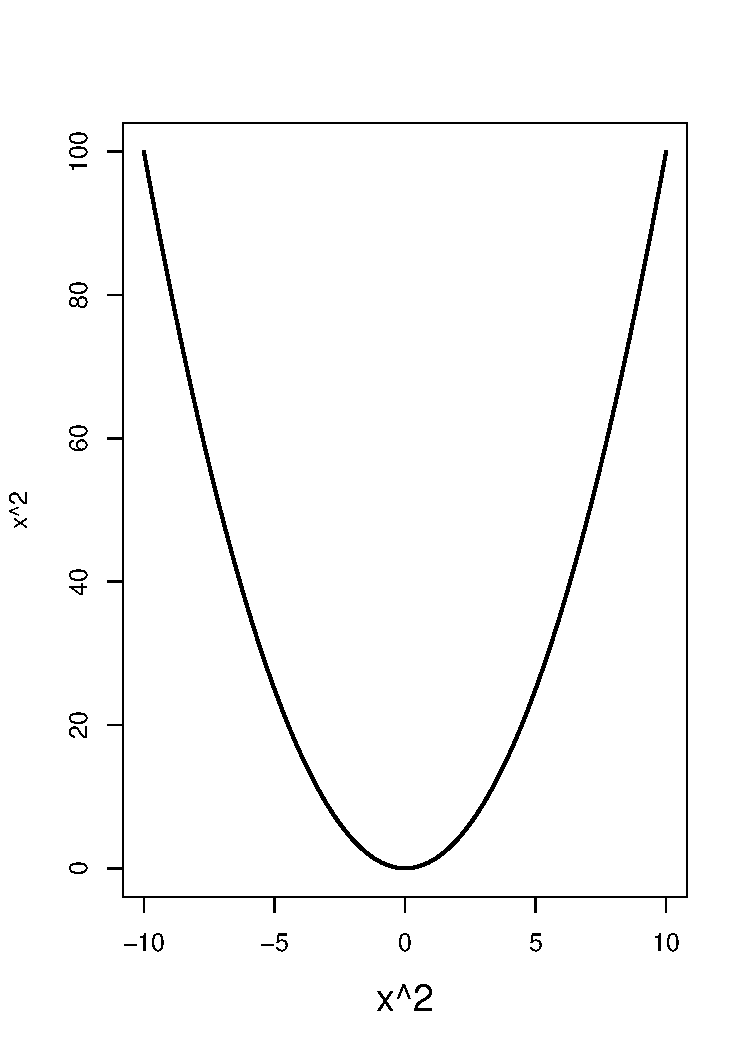
\includegraphics{TestAPB-x_y_squared}
\caption{Caption Test}
\label{Fig. 1}
\end{figure}

\end{document}
